The user is expected to have a working knowledge of \LaTeX. A good introduction is in~\cite{Oetiker2014}.  Its latest version can be accessed at \url{http://www.ctan.org/tex-archive/info/lshort}.




\section{Equations}
\label{sec:eqn_not}

The following examples show how to typeset equations in \LaTeX.  This section also shows examples of the use of \verb| \gls{ } | commands in conjunction with the items that are in the \verb| notation.tex | file. \textbf{Please make sure that the entries in} \verb| notation.tex |\textbf{  are those that are referenced in the \LaTeX \ document files used by this \documentType.  Please comment out unused notations and be careful with the commas and brackets  in} \verb| notation.tex |.

In~\eqref{eq:conv}, the output signal \gls{not:output_sigt} is the result of the convolution of the input signal \gls{not:input_sigt} and the impulse response \gls{not:ir}.

\begin{eqnarray}   
     y\left( t \right) = h\left( t \right) * x\left( t \right)=\int_{-\infty}^{+\infty}h\left( t-\tau \right)x\left( \tau \right) \mathrm{d}\tau
	\label{eq:conv}
\end{eqnarray}

Other example equations are as follows.

\begin{eqnarray}
	\left[ \dfrac{ V_{1} }{ I_{1} } \right] = 
	\begin{bmatrix}
		A & B \\ 
		C & D 
	\end{bmatrix} 
	\left[ \dfrac{ V_{2} }{ I_{2} } \right]
	\label{eq:ABCD}
\end{eqnarray}

\begin{eqnarray}
\dfrac{1}{2} < \left\lfloor \mathrm{mod}\left(\left\lfloor \dfrac{y}{17} \right\rfloor 2^{-17 \lfloor x \rfloor - \mathrm{mod}(\lfloor y\rfloor, 17)},2\right)\right\rfloor,
\end{eqnarray}

\begin{eqnarray}
| \zeta(x)^3 \zeta(x + iy)^4 \zeta(x + 2iy) | = 
\exp\sum_{n,p} \frac{3 + 4 \cos( ny \log p) + \cos (2ny \log p)}{np^{nx}} \ge 1
\end{eqnarray}

\newpage
The verbatim \LaTeX \ code of Sec.~\ref{sec:eqn_not} is in List.~\ref{lst:eqn_gls}.

\begin{lstlisting}[
float=h,
caption=Sample \LaTeX \ code for equations and notations usage, 
label=lst:eqn_gls,
language=TeX,
frame=single]
The following examples show how to typeset equations in \LaTeX. 

In~\eqref{eq:conv}, the output signal \gls{not:output_sigt} is the result of the convolution of the input signal \gls{not:input_sigt} and the impulse response \gls{not:ir}.

\begin{eqnarray}   
     y\left( t \right) = h\left( t \right) * x\left( t \right)=\int_{-\infty}^{+\infty}h\left( t-\tau \right)x\left( \tau \right) \mathrm{d}\tau
	\label{eq:conv}
\end{eqnarray}

Other example equations are as follows.

\begin{eqnarray}
	\left[ \dfrac{ V_{1} }{ I_{1} } \right] = 
	\begin{bmatrix}
		A & B \\ 
		C & D 
	\end{bmatrix} 
	\left[ \dfrac{ V_{2} }{ I_{2} } \right]
	\label{eq:ABCD}
\end{eqnarray}

\begin{eqnarray}
{1\over 2} < \left\lfloor \mathrm{mod}\left(\left\lfloor {y \over 17} \right\rfloor 2^{-17 \lfloor x \rfloor - \mathrm{mod}(\lfloor y\rfloor, 17)},2\right)\right\rfloor,
\end{eqnarray}

\begin{eqnarray}
| \zeta(x)^3\zeta(x+iy)^4\zeta(x+2iy) | = 
\exp\sum_{n,p}\frac{3+4\cos(ny\log p) +\cos (2ny\log p)}{np^{nx}}\ge 1
\end{eqnarray}
\end{lstlisting}
\cleardoublepage







\newpage
\section{Notations}
\label{sec:not}
In order to use the standardized notation, the user is highly suggested to see the ISO~80000-2 standard~\cite{ISO800002}. The following were taken from \verb| isomath-test.tex |.

% A teststring with Latin and Greek letters::
\newcommand{\teststring}{%
% capital Latin letters
% A,B,C,
A,B,
% capital Greek letters
%\Gamma,\Delta,\Theta,\Lambda,\Xi,\Pi,\Sigma,\Upsilon,\Phi,\Psi,
\Gamma,\Delta,\Theta,\Lambda,\Xi,\Pi,\Sigma,\Phi,\Psi,\Omega,
% small Greek letters
\alpha,\beta,\pi,\nu,\omega,
% small Latin letters:
% compare \nu, \omega, v, and w
v,w,
% digits
0,1,9
}


\subsection*{Math alphabets}

If there are other symbols in place of Greek letters in a math
alphabet, it uses T1 or OT1 font encoding instead of OML.

\begin{eqnarray*}
\mbox{mathnormal} &  & \teststring \\
\mbox{mathit} &  & \mathit{\teststring}\\
\mbox{mathrm} &  & \mathrm{\teststring}\\
\mbox{mathbf} &  & \mathbf{\teststring}\\
\mbox{mathsf} &  & \mathsf{\teststring}\\
\mbox{mathtt} &  & \mathtt{\teststring}
\end{eqnarray*}
 New alphabets bold-italic, sans-serif-italic, and sans-serif-bold-italic.
\begin{eqnarray*}
\mbox{mathbfit}     &  & \mathbfit{\teststring}\\
\mbox{mathsfit}     &  & \mathsfit{\teststring}\\
\mbox{mathsfbfit} &  & \mathsfbfit{\teststring}
\end{eqnarray*}
%
Do the math alphabets match?

$
\mathnormal  {a x \alpha \omega}
\mathbfit    {a x \alpha \omega}
\mathsfbfit{a x \alpha \omega}
\quad
\mathsfbfit{T C \Theta \Gamma}
\mathbfit    {T C \Theta \Gamma}
\mathnormal  {T C \Theta \Gamma}
$

\subsection*{Vector symbols}

Alphabetic symbols for vectors are boldface italic,
$\vec{\lambda}=\vec{e}_{1}\cdot\vec{a}$,
while numeric ones (e.g. the zero vector) are bold upright,
$\vec{a} + \vec{0} = \vec{a}$.

\subsection*{Matrix symbols}

Symbols for matrices are boldface italic, too:%
\footnote{However, matrix symbols are usually capital letters whereas vectors
are small ones. Exceptions are physical quantities like the force
vector $\vec{F}$ or the electrical field $\vec{E}$.%
}
$\matrixsym{\Lambda}=\matrixsym{E}\cdot\matrixsym{A}.$


\subsection*{Tensor symbols}

Symbols for tensors are sans-serif bold italic,

\[
   \tensorsym{\alpha}  =  \tensorsym{e}\cdot\tensorsym{a}
   \quad \Longleftrightarrow \quad
   \alpha_{ijl}  =  e_{ijk}\cdot a_{kl}.
\]


The permittivity tensor describes the coupling of electric field and
displacement: \[
\vec{D}=\epsilon_{0}\tensorsym{\epsilon}_{\mathrm{r}}\vec{E}\]



\newpage
\subsection*{Bold math version}

The ``bold'' math version is selected with the commands
\verb+\boldmath+ or \verb+\mathversion{bold}+

{\boldmath
	\begin{eqnarray*}
	\mbox{mathnormal} &  & \teststring \\
	\mbox{mathit} &  & \mathit{\teststring}\\
	\mbox{mathrm} &  & \mathrm{\teststring}\\
	\mbox{mathbf} &  & \mathbf{\teststring}\\
	\mbox{mathsf} &  & \mathsf{\teststring}\\
	\mbox{mathtt} &  & \mathtt{\teststring}
	\end{eqnarray*}
	 New alphabets bold-italic, sans-serif-italic, and sans-serif-bold-italic.
	\begin{eqnarray*}
	\mbox{mathbfit}     &  & \mathbfit{\teststring}\\
	\mbox{mathsfit}     &  & \mathsfit{\teststring}\\
	\mbox{mathsfbfit} &  & \mathsfbfit{\teststring}
	\end{eqnarray*}
	%
	Do the math alphabets match?

	$
	\mathnormal  {a x \alpha \omega}
	\mathbfit    {a x \alpha \omega}
	\mathsfbfit{a x \alpha \omega}
	\quad
	\mathsfbfit{T C \Theta \Gamma}
	\mathbfit    {T C \Theta \Gamma}
	\mathnormal  {T C \Theta \Gamma}
	$

	\subsection*{Vector symbols}

	Alphabetic symbols for vectors are boldface italic,
	$\vec{\lambda}=\vec{e}_{1}\cdot\vec{a}$,
	while numeric ones (e.g. the zero vector) are bold upright,
	$\vec{a} + \vec{0} = \vec{a}$.




	\subsection*{Matrix symbols}

	Symbols for matrices are boldface italic, too:%
	\footnote{However, matrix symbols are usually capital letters whereas vectors
	are small ones. Exceptions are physical quantities like the force
	vector $\vec{F}$ or the electrical field $\vec{E}$.%
	}
	$\matrixsym{\Lambda}=\matrixsym{E}\cdot\matrixsym{A}.$


	\subsection*{Tensor symbols}

	Symbols for tensors are sans-serif bold italic,

	\[
		 \tensorsym{\alpha}  =  \tensorsym{e}\cdot\tensorsym{a}
		 \quad \Longleftrightarrow \quad
		 \alpha_{ijl}  =  e_{ijk}\cdot a_{kl}.
	\]

	The permittivity tensor describes the coupling of electric field and
	displacement: \[
	\vec{D}=\epsilon_{0}\tensorsym{\epsilon}_{\mathrm{r}}\vec{E}\]
}











\newpage
The verbatim \LaTeX \ code of Sec.~\ref{sec:not} is in List.~\ref{lst:not}.

\begin{lstlisting}[
%float=h,% do not use float option for long listings
caption=Sample \LaTeX \ code for notations usage, 
label=lst:not,
language=TeX,
frame=single]
% A teststring with Latin and Greek letters::
\newcommand{\teststring}{%
% capital Latin letters
% A,B,C,
A,B,
% capital Greek letters
%\Gamma,\Delta,\Theta,\Lambda,\Xi,\Pi,\Sigma,\Upsilon,\Phi,\Psi,
\Gamma,\Delta,\Theta,\Lambda,\Xi,\Pi,\Sigma,\Phi,\Psi,\Omega,
% small Greek letters
\alpha,\beta,\pi,\nu,\omega,
% small Latin letters:
% compare \nu, \omega, v, and w
v,w,
% digits
0,1,9
}


\subsection*{Math alphabets}

If there are other symbols in place of Greek letters in a math
alphabet, it uses T1 or OT1 font encoding instead of OML.

\begin{eqnarray*}
\mbox{mathnormal} &  & \teststring \\
\mbox{mathit} &  & \mathit{\teststring}\\
\mbox{mathrm} &  & \mathrm{\teststring}\\
\mbox{mathbf} &  & \mathbf{\teststring}\\
\mbox{mathsf} &  & \mathsf{\teststring}\\
\mbox{mathtt} &  & \mathtt{\teststring}
\end{eqnarray*}
 New alphabets bold-italic, sans-serif-italic, and sans-serif-bold-italic.
\begin{eqnarray*}
\mbox{mathbfit}     &  & \mathbfit{\teststring}\\
\mbox{mathsfit}     &  & \mathsfit{\teststring}\\
\mbox{mathsfbfit} &  & \mathsfbfit{\teststring}
\end{eqnarray*}
%
Do the math alphabets match?

$
\mathnormal  {a x \alpha \omega}
\mathbfit    {a x \alpha \omega}
\mathsfbfit{a x \alpha \omega}
\quad
\mathsfbfit{T C \Theta \Gamma}
\mathbfit    {T C \Theta \Gamma}
\mathnormal  {T C \Theta \Gamma}
$

\subsection*{Vector symbols}

Alphabetic symbols for vectors are boldface italic,
$\vec{\lambda}=\vec{e}_{1}\cdot\vec{a}$,
while numeric ones (e.g. the zero vector) are bold upright,
$\vec{a} + \vec{0} = \vec{a}$.

\subsection*{Matrix symbols}

Symbols for matrices are boldface italic, too:%
\footnote{However, matrix symbols are usually capital letters whereas vectors
are small ones. Exceptions are physical quantities like the force
vector $\vec{F}$ or the electrical field $\vec{E}$.%
}
$\matrixsym{\Lambda}=\matrixsym{E}\cdot\matrixsym{A}.$


\subsection*{Tensor symbols}

Symbols for tensors are sans-serif bold italic,

\[
   \tensorsym{\alpha}  =  \tensorsym{e}\cdot\tensorsym{a}
   \quad \Longleftrightarrow \quad
   \alpha_{ijl}  =  e_{ijk}\cdot a_{kl}.
\]


The permittivity tensor describes the coupling of electric field and
displacement: \[
\vec{D}=\epsilon_{0}\tensorsym{\epsilon}_{\mathrm{r}}\vec{E}\]



\newpage
\subsection*{Bold math version}

The ``bold'' math version is selected with the commands
\verb+\boldmath+ or \verb+\mathversion{bold}+

{\boldmath
	\begin{eqnarray*}
	\mbox{mathnormal} &  & \teststring \\
	\mbox{mathit} &  & \mathit{\teststring}\\
	\mbox{mathrm} &  & \mathrm{\teststring}\\
	\mbox{mathbf} &  & \mathbf{\teststring}\\
	\mbox{mathsf} &  & \mathsf{\teststring}\\
	\mbox{mathtt} &  & \mathtt{\teststring}
	\end{eqnarray*}
	 New alphabets bold-italic, sans-serif-italic, and sans-serif-bold-italic.
	\begin{eqnarray*}
	\mbox{mathbfit}     &  & \mathbfit{\teststring}\\
	\mbox{mathsfit}     &  & \mathsfit{\teststring}\\
	\mbox{mathsfbfit} &  & \mathsfbfit{\teststring}
	\end{eqnarray*}
	%
	Do the math alphabets match?

	$
	\mathnormal  {a x \alpha \omega}
	\mathbfit    {a x \alpha \omega}
	\mathsfbfit{a x \alpha \omega}
	\quad
	\mathsfbfit{T C \Theta \Gamma}
	\mathbfit    {T C \Theta \Gamma}
	\mathnormal  {T C \Theta \Gamma}
	$

	\subsection*{Vector symbols}

	Alphabetic symbols for vectors are boldface italic,
	$\vec{\lambda}=\vec{e}_{1}\cdot\vec{a}$,
	while numeric ones (e.g. the zero vector) are bold upright,
	$\vec{a} + \vec{0} = \vec{a}$.




	\subsection*{Matrix symbols}

	Symbols for matrices are boldface italic, too:%
	\footnote{However, matrix symbols are usually capital letters whereas vectors
	are small ones. Exceptions are physical quantities like the force
	vector $\vec{F}$ or the electrical field $\vec{E}$.%
	}
	$\matrixsym{\Lambda}=\matrixsym{E}\cdot\matrixsym{A}.$


	\subsection*{Tensor symbols}

	Symbols for tensors are sans-serif bold italic,

	\[
		 \tensorsym{\alpha}  =  \tensorsym{e}\cdot\tensorsym{a}
		 \quad \Longleftrightarrow \quad
		 \alpha_{ijl}  =  e_{ijk}\cdot a_{kl}.
	\]

	The permittivity tensor describes the coupling of electric field and
	displacement: \[
	\vec{D}=\epsilon_{0}\tensorsym{\epsilon}_{\mathrm{r}}\vec{E}\]
}

\end{lstlisting}
\cleardoublepage











\newpage
\section{Abbreviation}\
\label{sec:abbrv}

This section shows examples of the use of \LaTeX commands in conjunction with the items that are in the \verb| abbreviation.tex | and in the \verb| glossary.tex | files.  Please see List.~\ref{lst:abbrv}. \textbf{To lessen the \LaTeX \ compilation time, it is suggested that you use} \verb| \acr{ } | \textbf{only for the first occurrence of the word to be abbreviated.}

Again please see List.~\ref{lst:abbrv}. Here is an example of first use: \acr{ac}. Next use: \acr{ac}. Full: \gls{ac}.  Here's an acronym referenced using \verb| \acr |: \acr{html}.  And here it is again: \acr{html}. If you are used to the \texttt{glossaries} package, note the difference in using \verb| \gls |: \gls{html}. And again (no difference): \gls{html}. Here are some more entries:

\begin{itemize}

	\item \acr{xml} and \acr{css}.

	\item Next use: \acr{xml} and \acr{css}.

	\item Full form: \gls{xml} and \gls{css}.

	\item Reset again. \glsresetall{abbreviation}

	\item Start with a capital. \Acr{html}.

	\item Next: \Acr{html}. Full: \Gls{html}.

	\item Prefer capitals? \renewcommand{\acronymfont}[1]{\MakeTextUppercase{#1}} \Acr{xml}. Next: \acr{xml}. Full: \gls{xml}.

	\item Prefer small-caps? \renewcommand{\acronymfont}[1]{\textsc{#1}} \Acr{css}. Next: \acr{css}. Full: \gls{css}.

	\item Resetting all acronyms.\glsresetall{abbreviation}

	\item Here are the acronyms again:

	\item \Acr{html}, \acr{xml} and \acr{css}.

	\item Next use: \Acr{html}, \acr{xml} and \acr{css}.

	\item Full form: \Gls{html}, \gls{xml} and \gls{css}.

	\item Provide your own link text: \glslink{[textbf]css}{style sheet}.

\end{itemize}



The verbatim \LaTeX \ code of Sec.~\ref{sec:abbrv} is in List.~\ref{lst:abbrv}.

\begin{lstlisting}[
float=h,
caption=Sample \LaTeX \ code for abbreviations usage, 
label=lst:abbrv,
language=TeX,
frame=single]
Again please see List.~\ref{lst:abbrv}. Here is an example of first use: \acr{ac}. Next use: \acr{ac}. Full: \gls{ac}.  Here's an acronym referenced using \verb| \acr |: \acr{html}.  And here it is again: \acr{html}. If you are used to the \texttt{glossaries} package, note the difference in using \verb| \gls |: \gls{html}. And again (no difference): \gls{html}. Here are some more entries:

\begin{itemize}

	\item \acr{xml} and \acr{css}.

	\item Next use: \acr{xml} and \acr{css}.

	\item Full form: \gls{xml} and \gls{css}.

	\item Reset again. \glsresetall{abbreviation}

	\item Start with a capital. \Acr{html}.

	\item Next: \Acr{html}. Full: \Gls{html}.

	\item Prefer capitals? \renewcommand{\acronymfont}[1]{\MakeTextUppercase{#1}} \Acr{xml}. Next: \acr{xml}. Full: \gls{xml}.

	\item Prefer small-caps? \renewcommand{\acronymfont}[1]{\textsc{#1}} \Acr{css}. Next: \acr{css}. Full: \gls{css}.

	\item Resetting all acronyms.\glsresetall{abbreviation}

	\item Here are the acronyms again:

	\item \Acr{html}, \acr{xml} and \acr{css}.

	\item Next use: \Acr{html}, \acr{xml} and \acr{css}.

	\item Full form: \Gls{html}, \gls{xml} and \gls{css}.

	\item Provide your own link text: \glslink{[textbf]css}{style} 
	
\end{itemize}
\end{lstlisting}
\cleardoublepage






\newpage
\section{Glossary}
\label{sec:glos}

This section shows examples of the use of \verb| \gls{ } | commands in conjunction with the items that are in the \verb| glossary.tex | and \verb| notation.tex | files.  Note that entries in  \verb| notation.tex |  are prefixed with ``\verb| not: |'' label (see List.~\ref{lst:glos}).

\textbf{Please make sure that the entries in} \verb| notation.tex |\textbf{  are those that are referenced in the \LaTeX \ document files used by this \documentType.  Please comment out unused notations and be careful with the commas and brackets  in} \verb| notation.tex |.

\begin{itemize}

	\item \Glspl{matrix} are usually denoted by a bold capital letter, such as $\mathbfit{A}$. The \gls{matrix}'s $(i,j)$th element is usually denoted $a_{ij}$. \Gls{matrix} $\mathbf{I}$ is the identity \gls{matrix}.

	\item A set, denoted as \gls{not:set}, is a collection of objects.

	\item The universal set,  denoted as \gls{not:universalSet}, is the set of everything.

	\item The empty set, denoted as \gls{not:emptySet}, contains no elements.

	\item The cardinality of a set, denoted as \gls{not:cardinality}, is the number of elements in the set.

\end{itemize}


The verbatim \LaTeX \ code for the part of Sec.~\ref{sec:glos} is in List.~\ref{lst:glos}.

\begin{lstlisting}[
float=h,
caption=Sample \LaTeX \ code for glossary and notations usage, 
label=lst:glos,
language=TeX,
frame=single]
\begin{itemize}

	\item \Glspl{matrix} are usually denoted by a bold capital letter, such as $\mathbfit{A}$. The \gls{matrix}'s $(i,j)$th element is usually denoted $a_{ij}$. \Gls{matrix} $\mathbf{I}$ is the identity \gls{matrix}.

	\item A set, denoted as \gls{not:set}, is a collection of objects.

	\item The universal set,  denoted as \gls{not:universalSet}, is the set of everything.

	\item The empty set, denoted as \gls{not:emptySet}, contains no elements.

	\item The cardinality of a set, denoted as \gls{not:cardinality}, is the number of elements in the set.

\end{enumerate}
\end{lstlisting}
\cleardoublepage












\newpage
\section{Figure}

This section shows several ways of placing figures.  PDF\LaTeX \ compatible files are PDF, PNG, and JPG.  Please see the \verb| figure | subdirectory.

\begin{figure}[!htbp]
	\centering
		
\includegraphics[width=0.5\textwidth]{example}
	\caption{A quadrilateral image example.}
	\label{fig:example}
\end{figure}
\cleardoublepage

Fig.~\ref{fig:example} is a gray box enclosed by a dark border. List.~\ref{lst:onefig} shows the corresponding \LaTeX \ code. 


\begin{lstlisting}[
float=h,
caption=Sample \LaTeX \ code for a single figure, 
label=lst:onefig,
language=TeX,
frame=single]
\begin{figure}[!htbp]
	\centering
		
\includegraphics[width=0.5\textwidth]{example}
	\caption{A quadrilateral image example.}
	\label{fig:example}
\end{figure}
\cleardoublepage

Fig.~\ref{fig:example} is a gray box enclosed by a dark border. List.~\ref{lst:onefig} shows the corresponding \LaTeX \ code. 	
\end{figure}
\end{lstlisting}
\cleardoublepage





\begin{figure}[!htbp]
\centering
\subbottom[A sub-figure in the top row.]{

\includegraphics[width=0.35\textwidth]{example}
\label{fig:top}
}
\vfill
\subbottom[A sub-figure in the middle row.]{

\includegraphics[width=0.35\textwidth]{example}
\label{fig:mid}
}
\vfill
\subbottom[A sub-figure in the bottom row.]{

\includegraphics[width=0.35\textwidth]{example}
\label{fig:botm}
}
\caption{Figures on top of each other. See List.~\ref{lst:figsontop} for the corresponding \LaTeX \ code. } 
\label{fig:tmb}
\end{figure}
\cleardoublepage




\begin{lstlisting}[
float=h,
caption=Sample \LaTeX \ code for three figures on top of each other, 
label=lst:figsontop,
language=TeX,
frame=single]
\begin{figure}[!htbp]
\centering
\subbottom[A sub-figure in the top row.]{

\includegraphics[width=0.35\textwidth]{example}
\label{fig:top}
}
\vfill
\subbottom[A sub-figure in the middle row.]{

\includegraphics[width=0.35\textwidth]{example}
\label{fig:mid}
}
\vfill
\subbottom[A sub-figure in the bottom row.]{

\includegraphics[width=0.35\textwidth]{example}
\label{fig:botm}
}
\caption{Figures on top of each other} 
\label{fig:tmb}
\end{figure}
\end{lstlisting}
\cleardoublepage







\begin{figure}[!htbp]
\centering
\subbottom[A sub-figure in the upper-left corner.]{

\includegraphics[width=0.45\textwidth]{example}
\label{fig:upprleft}
}
\hfill
\subbottom[A sub-figure in the upper-right corner.]{

\includegraphics[width=0.45\textwidth]{example}
\label{fig:uppright}
}
\vfill
\subbottom[A sub-figure in the lower-left corner.]{

\includegraphics[width=0.45\textwidth]{example}
\label{fig:lowerleft}
}
\hfill
\subbottom[A sub-figure in the lower-right corner]{

\includegraphics[width=0.45\textwidth]{example}
\label{fig:lowright}
}
\caption{Four figures in each corner. See List.~\ref{lst:fourfigs} for the corresponding \LaTeX \ code.} 
\label{fig:fourfig}
\end{figure}
\cleardoublepage




\begin{lstlisting}[
float=h,
caption=Sample \LaTeX \ code for the four figures, 
label=lst:fourfigs,
language=TeX,
frame=single]
\begin{figure}[!htbp]
\centering
\subbottom[A sub-figure in the upper-left corner.]{

\includegraphics[width=0.45\textwidth]{example}
\label{fig:upprleft}
}
\hfill
\subbottom[A sub-figure in the upper-right corner.]{

\includegraphics[width=0.45\textwidth]{example}
\label{fig:uppright}
}
\vfill
\subbottom[A sub-figure in the lower-left corner.]{

\includegraphics[width=0.45\textwidth]{example}
\label{fig:lowerleft}
}
\hfill
\subbottom[A sub-figure in the lower-right corner]{

\includegraphics[width=0.45\textwidth]{example}
\label{fig:lowright}
}
\caption{Four figures in each corner. See List.~\ref{lst:fourfigs} for the corresponding \LaTeX \ code.} 
\label{fig:fourfig}
\end{figure}
\end{lstlisting}
\cleardoublepage





\newpage
\section{Table}

This section shows an example of placing a table (a long one). Table~\ref{tab:triple_grid} are the triples. 

\begin{center}
{\scriptsize
\begin{tabularx}{\textwidth}{p{0.1\textwidth}|p{0.2\textwidth}|p{0.5\textwidth}}
\caption{Feasible triples for highly variable grid} \label{tab:triple_grid} \\
\hline 
\hline 
\textbf{Time (s)} & 
\textbf{Triple chosen} & 
\textbf{Other feasible triples} \\ 
\hline 
\endfirsthead
\multicolumn{3}{c}%
{\textit{Continued from previous page}} \\
\hline
\hline 
\textbf{Time (s)} & 
\textbf{Triple chosen} & 
\textbf{Other feasible triples} \\ 
\hline 
\endhead
\hline 
\multicolumn{3}{r}{\textit{Continued on next page}} \\ 
\endfoot
\hline 
\endlastfoot
\hline

0 & (1, 11, 13725) & (1, 12, 10980), (1, 13, 8235), (2, 2, 0), (3, 1, 0) \\
2745 & (1, 12, 10980) & (1, 13, 8235), (2, 2, 0), (2, 3, 0), (3, 1, 0) \\
5490 & (1, 12, 13725) & (2, 2, 2745), (2, 3, 0), (3, 1, 0) \\
8235 & (1, 12, 16470) & (1, 13, 13725), (2, 2, 2745), (2, 3, 0), (3, 1, 0) \\
10980 & (1, 12, 16470) & (1, 13, 13725), (2, 2, 2745), (2, 3, 0), (3, 1, 0) \\
13725 & (1, 12, 16470) & (1, 13, 13725), (2, 2, 2745), (2, 3, 0), (3, 1, 0) \\
16470 & (1, 13, 16470) & (2, 2, 2745), (2, 3, 0), (3, 1, 0) \\
19215 & (1, 12, 16470) & (1, 13, 13725), (2, 2, 2745), (2, 3, 0), (3, 1, 0) \\
21960 & (1, 12, 16470) & (1, 13, 13725), (2, 2, 2745), (2, 3, 0), (3, 1, 0) \\
24705 & (1, 12, 16470) & (1, 13, 13725), (2, 2, 2745), (2, 3, 0), (3, 1, 0) \\
27450 & (1, 12, 16470) & (1, 13, 13725), (2, 2, 2745), (2, 3, 0), (3, 1, 0) \\
30195 & (2, 2, 2745) & (2, 3, 0), (3, 1, 0) \\
32940 & (1, 13, 16470) & (2, 2, 2745), (2, 3, 0), (3, 1, 0) \\
35685 & (1, 13, 13725) & (2, 2, 2745), (2, 3, 0), (3, 1, 0) \\
38430 & (1, 13, 10980) & (2, 2, 2745), (2, 3, 0), (3, 1, 0) \\
41175 & (1, 12, 13725) & (1, 13, 10980), (2, 2, 2745), (2, 3, 0), (3, 1, 0) \\
43920 & (1, 13, 10980) & (2, 2, 2745), (2, 3, 0), (3, 1, 0) \\
46665 & (2, 2, 2745) & (2, 3, 0), (3, 1, 0) \\
49410 & (2, 2, 2745) & (2, 3, 0), (3, 1, 0) \\
52155 & (1, 12, 16470) & (1, 13, 13725), (2, 2, 2745), (2, 3, 0), (3, 1, 0) \\
54900 & (1, 13, 13725) & (2, 2, 2745), (2, 3, 0), (3, 1, 0) \\
57645 & (1, 13, 13725) & (2, 2, 2745), (2, 3, 0), (3, 1, 0) \\
60390 & (1, 12, 13725) & (2, 2, 2745), (2, 3, 0), (3, 1, 0) \\
63135 & (1, 13, 16470) & (2, 2, 2745), (2, 3, 0), (3, 1, 0) \\
65880 & (1, 13, 16470) & (2, 2, 2745), (2, 3, 0), (3, 1, 0) \\
68625 & (2, 2, 2745) & (2, 3, 0), (3, 1, 0) \\
71370 & (1, 13, 13725) & (2, 2, 2745), (2, 3, 0), (3, 1, 0) \\
74115 & (1, 12, 13725) & (2, 2, 2745), (2, 3, 0), (3, 1, 0) \\
76860 & (1, 13, 13725) & (2, 2, 2745), (2, 3, 0), (3, 1, 0) \\
79605 & (1, 13, 13725) & (2, 2, 2745), (2, 3, 0), (3, 1, 0) \\
82350 & (1, 12, 13725) & (2, 2, 2745), (2, 3, 0), (3, 1, 0) \\
85095 & (1, 12, 13725) & (1, 13, 10980), (2, 2, 2745), (2, 3, 0), (3, 1, 0) \\
87840 & (1, 13, 16470) & (2, 2, 2745), (2, 3, 0), (3, 1, 0) \\
90585 & (1, 13, 16470) & (2, 2, 2745), (2, 3, 0), (3, 1, 0) \\
93330 & (1, 13, 13725) & (2, 2, 2745), (2, 3, 0), (3, 1, 0) \\
96075 & (1, 13, 16470) & (2, 2, 2745), (2, 3, 0), (3, 1, 0) \\
98820 & (1, 13, 16470) & (2, 2, 2745), (2, 3, 0), (3, 1, 0) \\
101565 & (1, 13, 13725) & (2, 2, 2745), (2, 3, 0), (3, 1, 0) \\
104310 & (1, 13, 16470) & (2, 2, 2745), (2, 3, 0), (3, 1, 0) \\
107055 & (1, 13, 13725) & (2, 2, 2745), (2, 3, 0), (3, 1, 0) \\
109800 & (1, 13, 13725) & (2, 2, 2745), (2, 3, 0), (3, 1, 0) \\
112545 & (1, 12, 16470) & (1, 13, 13725), (2, 2, 2745), (2, 3, 0), (3, 1, 0) \\
115290 & (1, 13, 16470) & (2, 2, 2745), (2, 3, 0), (3, 1, 0) \\
118035 & (1, 13, 13725) & (2, 2, 2745), (2, 3, 0), (3, 1, 0) \\
120780 & (1, 13, 16470) & (2, 2, 2745), (2, 3, 0), (3, 1, 0) \\
123525 & (1, 13, 13725) & (2, 2, 2745), (2, 3, 0), (3, 1, 0) \\
126270 & (1, 12, 16470) & (1, 13, 13725), (2, 2, 2745), (2, 3, 0), (3, 1, 0) \\
129015 & (2, 2, 2745) & (2, 3, 0), (3, 1, 0) \\
131760 & (2, 2, 2745) & (2, 3, 0), (3, 1, 0) \\
134505 & (1, 13, 16470) & (2, 2, 2745), (2, 3, 0), (3, 1, 0) \\
137250 & (1, 13, 13725) & (2, 2, 2745), (2, 3, 0), (3, 1, 0) \\
139995 & (2, 2, 2745) & (2, 3, 0), (3, 1, 0) \\
142740 & (2, 2, 2745) & (2, 3, 0), (3, 1, 0) \\
145485 & (1, 12, 16470) & (1, 13, 13725), (2, 2, 2745), (2, 3, 0), (3, 1, 0) \\
148230 & (2, 2, 2745) & (2, 3, 0), (3, 1, 0) \\
150975 & (1, 13, 16470) & (2, 2, 2745), (2, 3, 0), (3, 1, 0) \\
153720 & (1, 12, 13725) & (2, 2, 2745), (2, 3, 0), (3, 1, 0) \\
156465 & (1, 13, 13725) & (2, 2, 2745), (2, 3, 0), (3, 1, 0) \\
159210 & (1, 13, 13725) & (2, 2, 2745), (2, 3, 0), (3, 1, 0) \\
161955 & (1, 13, 16470) & (2, 2, 2745), (2, 3, 0), (3, 1, 0) \\
164700 & (1, 13, 13725) & (2, 2, 2745), (2, 3, 0), (3, 1, 0) \\
\end{tabularx}
}
\end{center}
\cleardoublepage









List.~\ref{lst:tabl} shows the corresponding \LaTeX \ code. 

\begin{lstlisting}[
%float=h,% do not use float option for long listings
caption=Sample \LaTeX \ code for making typical table environment, 
label=lst:tabl,
language=TeX,
frame=single,]
\begin{center}
{\scriptsize
\begin{tabularx}{\textwidth}{p{0.1\textwidth}|p{0.2\textwidth}|p{0.5\textwidth}}
\caption{Feasible triples for highly variable grid} \label{tab:triple_grid} \\
\hline 
\hline 
\textbf{Time (s)} & 
\textbf{Triple chosen} & 
\textbf{Other feasible triples} \\ 
\hline 
\endfirsthead
\multicolumn{3}{c}%
{\textit{Continued from previous page}} \\
\hline
\hline 
\textbf{Time (s)} & 
\textbf{Triple chosen} & 
\textbf{Other feasible triples} \\ 
\hline 
\endhead
\hline 
\multicolumn{3}{r}{\textit{Continued on next page}} \\ 
\endfoot
\hline 
\endlastfoot
\hline

0 & (1, 11, 13725) & (1, 12, 10980), (1, 13, 8235), (2, 2, 0), (3, 1, 0) \\
2745 & (1, 12, 10980) & (1, 13, 8235), (2, 2, 0), (2, 3, 0), (3, 1, 0) \\
5490 & (1, 12, 13725) & (2, 2, 2745), (2, 3, 0), (3, 1, 0) \\
8235 & (1, 12, 16470) & (1, 13, 13725), (2, 2, 2745), (2, 3, 0), (3, 1, 0) \\
10980 & (1, 12, 16470) & (1, 13, 13725), (2, 2, 2745), (2, 3, 0), (3, 1, 0) \\
13725 & (1, 12, 16470) & (1, 13, 13725), (2, 2, 2745), (2, 3, 0), (3, 1, 0) \\
16470 & (1, 13, 16470) & (2, 2, 2745), (2, 3, 0), (3, 1, 0) \\
19215 & (1, 12, 16470) & (1, 13, 13725), (2, 2, 2745), (2, 3, 0), (3, 1, 0) \\
21960 & (1, 12, 16470) & (1, 13, 13725), (2, 2, 2745), (2, 3, 0), (3, 1, 0) \\
24705 & (1, 12, 16470) & (1, 13, 13725), (2, 2, 2745), (2, 3, 0), (3, 1, 0) \\
27450 & (1, 12, 16470) & (1, 13, 13725), (2, 2, 2745), (2, 3, 0), (3, 1, 0) \\
30195 & (2, 2, 2745) & (2, 3, 0), (3, 1, 0) \\
32940 & (1, 13, 16470) & (2, 2, 2745), (2, 3, 0), (3, 1, 0) \\
35685 & (1, 13, 13725) & (2, 2, 2745), (2, 3, 0), (3, 1, 0) \\
38430 & (1, 13, 10980) & (2, 2, 2745), (2, 3, 0), (3, 1, 0) \\
41175 & (1, 12, 13725) & (1, 13, 10980), (2, 2, 2745), (2, 3, 0), (3, 1, 0) \\
43920 & (1, 13, 10980) & (2, 2, 2745), (2, 3, 0), (3, 1, 0) \\
46665 & (2, 2, 2745) & (2, 3, 0), (3, 1, 0) \\
49410 & (2, 2, 2745) & (2, 3, 0), (3, 1, 0) \\
52155 & (1, 12, 16470) & (1, 13, 13725), (2, 2, 2745), (2, 3, 0), (3, 1, 0) \\
54900 & (1, 13, 13725) & (2, 2, 2745), (2, 3, 0), (3, 1, 0) \\
57645 & (1, 13, 13725) & (2, 2, 2745), (2, 3, 0), (3, 1, 0) \\
60390 & (1, 12, 13725) & (2, 2, 2745), (2, 3, 0), (3, 1, 0) \\
63135 & (1, 13, 16470) & (2, 2, 2745), (2, 3, 0), (3, 1, 0) \\
65880 & (1, 13, 16470) & (2, 2, 2745), (2, 3, 0), (3, 1, 0) \\
68625 & (2, 2, 2745) & (2, 3, 0), (3, 1, 0) \\
71370 & (1, 13, 13725) & (2, 2, 2745), (2, 3, 0), (3, 1, 0) \\
74115 & (1, 12, 13725) & (2, 2, 2745), (2, 3, 0), (3, 1, 0) \\
76860 & (1, 13, 13725) & (2, 2, 2745), (2, 3, 0), (3, 1, 0) \\
79605 & (1, 13, 13725) & (2, 2, 2745), (2, 3, 0), (3, 1, 0) \\
82350 & (1, 12, 13725) & (2, 2, 2745), (2, 3, 0), (3, 1, 0) \\
85095 & (1, 12, 13725) & (1, 13, 10980), (2, 2, 2745), (2, 3, 0), (3, 1, 0) \\
87840 & (1, 13, 16470) & (2, 2, 2745), (2, 3, 0), (3, 1, 0) \\
90585 & (1, 13, 16470) & (2, 2, 2745), (2, 3, 0), (3, 1, 0) \\
93330 & (1, 13, 13725) & (2, 2, 2745), (2, 3, 0), (3, 1, 0) \\
96075 & (1, 13, 16470) & (2, 2, 2745), (2, 3, 0), (3, 1, 0) \\
98820 & (1, 13, 16470) & (2, 2, 2745), (2, 3, 0), (3, 1, 0) \\
101565 & (1, 13, 13725) & (2, 2, 2745), (2, 3, 0), (3, 1, 0) \\
104310 & (1, 13, 16470) & (2, 2, 2745), (2, 3, 0), (3, 1, 0) \\
107055 & (1, 13, 13725) & (2, 2, 2745), (2, 3, 0), (3, 1, 0) \\
109800 & (1, 13, 13725) & (2, 2, 2745), (2, 3, 0), (3, 1, 0) \\
112545 & (1, 12, 16470) & (1, 13, 13725), (2, 2, 2745), (2, 3, 0), (3, 1, 0) \\
115290 & (1, 13, 16470) & (2, 2, 2745), (2, 3, 0), (3, 1, 0) \\
118035 & (1, 13, 13725) & (2, 2, 2745), (2, 3, 0), (3, 1, 0) \\
120780 & (1, 13, 16470) & (2, 2, 2745), (2, 3, 0), (3, 1, 0) \\
123525 & (1, 13, 13725) & (2, 2, 2745), (2, 3, 0), (3, 1, 0) \\
126270 & (1, 12, 16470) & (1, 13, 13725), (2, 2, 2745), (2, 3, 0), (3, 1, 0) \\
129015 & (2, 2, 2745) & (2, 3, 0), (3, 1, 0) \\
131760 & (2, 2, 2745) & (2, 3, 0), (3, 1, 0) \\
134505 & (1, 13, 16470) & (2, 2, 2745), (2, 3, 0), (3, 1, 0) \\
137250 & (1, 13, 13725) & (2, 2, 2745), (2, 3, 0), (3, 1, 0) \\
139995 & (2, 2, 2745) & (2, 3, 0), (3, 1, 0) \\
142740 & (2, 2, 2745) & (2, 3, 0), (3, 1, 0) \\
145485 & (1, 12, 16470) & (1, 13, 13725), (2, 2, 2745), (2, 3, 0), (3, 1, 0) \\
148230 & (2, 2, 2745) & (2, 3, 0), (3, 1, 0) \\
150975 & (1, 13, 16470) & (2, 2, 2745), (2, 3, 0), (3, 1, 0) \\
153720 & (1, 12, 13725) & (2, 2, 2745), (2, 3, 0), (3, 1, 0) \\
156465 & (1, 13, 13725) & (2, 2, 2745), (2, 3, 0), (3, 1, 0) \\
159210 & (1, 13, 13725) & (2, 2, 2745), (2, 3, 0), (3, 1, 0) \\
161955 & (1, 13, 16470) & (2, 2, 2745), (2, 3, 0), (3, 1, 0) \\
164700 & (1, 13, 13725) & (2, 2, 2745), (2, 3, 0), (3, 1, 0) \\
\end{tabularx}
}
\end{center} 
\end{lstlisting}
\cleardoublepage








\newpage
\section{Algorithm or Pseudocode Listing}

Table~\ref{tab:calcxn} shows an example pseudocode.  Note that if the pseudocode exceeds one page, it can mean that its implementation is not modular.  List.~\ref{lst:algo} shows the corresponding \LaTeX \ code. 

\begin{table}[!htbp]
	\caption{Calculation of $y = x^n$}
	\label{tab:calcxn}
	{\footnotesize
	\begin{tabular}{lll}
	\hline
	\hline
	{\bfseries Input(s):} & & \\
	$n$ & : & $n$th power; $n \in \mathbb{Z}^{+}$ \\
	$x$ & : & base value; $x \in \mathbb{R}^{+}$ \\
	\hline
	{\bfseries Output(s):} & & \\
	$y$ & : & result; $y \in \mathbb{R}^{+}$  \\
	\hline
	\hline
	\\
	\end{tabular}
	}
	\begin{algorithmic}[1]
	{\footnotesize
		\REQUIRE $n \geq 0 \vee x \neq 0$
		\ENSURE $y = x^n$
		\STATE $y \Leftarrow 1$
		\IF{$n < 0$}
				\STATE $X \Leftarrow 1 / x$
				\STATE $N \Leftarrow -n$
		\ELSE
				\STATE $X \Leftarrow x$
				\STATE $N \Leftarrow n$
		\ENDIF
		\WHILE{$N \neq 0$}
				\IF{$N$ is even}
						\STATE $X \Leftarrow X \times X$
						\STATE $N \Leftarrow N / 2$
				\ELSE[$N$ is odd]
						\STATE $y \Leftarrow y \times X$
						\STATE $N \Leftarrow N - 1$
				\ENDIF
		\ENDWHILE
	}	
	\end{algorithmic}
\end{table}
\cleardoublepage




\begin{lstlisting}[
float=h,
caption=Sample \LaTeX \ code for algorithm or pseudocode listing usage, 
label=lst:algo,
language=TeX,
frame=single]
\begin{table}[!htbp]
	\caption{Calculation of $y = x^n$}
	\label{tab:calcxn}
	{\footnotesize
	\begin{tabular}{lll}
	\hline
	\hline
	{\bfseries Input(s):} & & \\
	$n$ & : & $n$th power; $n \in \mathbb{Z}^{+}$ \\
	$x$ & : & base value; $x \in \mathbb{R}^{+}$ \\
	\hline
	{\bfseries Output(s):} & & \\
	$y$ & : & result; $y \in \mathbb{R}^{+}$  \\
	\hline
	\hline
	\\
	\end{tabular}
	}
	\begin{algorithmic}[1]
	{\footnotesize
		\REQUIRE $n \geq 0 \vee x \neq 0$
		\ENSURE $y = x^n$
		\STATE $y \Leftarrow 1$
		\IF{$n < 0$}
				\STATE $X \Leftarrow 1 / x$
				\STATE $N \Leftarrow -n$
		\ELSE
				\STATE $X \Leftarrow x$
				\STATE $N \Leftarrow n$
		\ENDIF
		\WHILE{$N \neq 0$}
				\IF{$N$ is even}
						\STATE $X \Leftarrow X \times X$
						\STATE $N \Leftarrow N / 2$
				\ELSE[$N$ is odd]
						\STATE $y \Leftarrow y \times X$
						\STATE $N \Leftarrow N - 1$
				\ENDIF
		\ENDWHILE
	}	
	\end{algorithmic}
\end{table}
\end{lstlisting}
\cleardoublepage




\newpage
\section{Program/Code Listing}

List.~\ref{lst:fib_c} is a program listing of a C code for computing Fibonacci numbers by calling the actual code. Please see the \verb| code | subdirectory.

\lstinputlisting[
float=h,
caption={[Computing Fibonacci numbers]Computing Fibonacci numbers in C (\lstname) }, 
label=lst:fib_c, 
language=C,
frame=single]{./code/fibo.c}	

List.~\ref{lst:proglist} shows the corresponding \LaTeX \ code. 

\begin{lstlisting}[
float=h,
caption=Sample \LaTeX \ code for program listing, 
label=lst:proglist,
language=TeX,
frame=single]
List.~\ref{lst:fib_c} is a program listing of a C code for computing Fibonacci numbers by calling the actual code. Please see the \verb| code | subdirectory. 
\end{lstlisting}
\cleardoublepage









\newpage
\section{Referencing}
\label{sec:ref}

Referencing chapters: This appendix is in Appendix~\ref{ch:usage_examples}, which is about examples in using various \LaTeX \ commands.

Referencing sections: This section is Sec.~\ref{sec:ref}, which shows how to refer to the locations of various labels that have been placed in the \LaTeX \ files. List.~\ref{lst:refsec} shows the corresponding \LaTeX \ code. 

\begin{lstlisting}[
float=h,
caption=Sample \LaTeX \ code for referencing sections, 
label=lst:refsec,
language=TeX,
frame=single]
Referencing sections: This section is Sec.~\ref{sec:ref}, which shows how to refer to the locations of various labels that have been placed in the \LaTeX \ files. List.~\ref{lst:refsec} shows the corresponding \LaTeX \ code.  
\end{lstlisting}
\blindtext
\cleardoublepage






\subsection{A subsection}
\label{sec:subsec}

Referencing subsections: This section is Sec.~\ref{sec:subsec}, which shows how to refer to a subsection. List.~\ref{lst:refsub} shows the corresponding \LaTeX \ code. 

\begin{lstlisting}[
float=h,
caption=Sample \LaTeX \ code for referencing subsections, 
label=lst:refsub,
language=TeX,
frame=single]
Referencing subsections: This section is Sec.~\ref{sec:subsec}, which shows how to refer to a subsection. List.~\ref{lst:refsub} shows the corresponding \LaTeX \ code. 
\end{lstlisting} 
\blindtext
\cleardoublepage





\subsubsection{A sub-subsection}
\label{sec:subsubsec}


Referencing sub-subsections: This section is Sec.~\ref{sec:subsubsec}, which shows how to refer to a sub-subsection.  List.~\ref{lst:refsubsub} shows the corresponding \LaTeX \ code. 

\begin{lstlisting}[
float=h,
caption=Sample \LaTeX \ code for referencing sub-subsections, 
label=lst:refsubsub,
language=TeX,
frame=single]
Referencing sub-subsections: This section is Sec.~\ref{sec:subsubsec}, which shows how to refer to a sub-subsection. List.~\ref{lst:refsubsub} shows the corresponding \LaTeX \ code. 
\end{lstlisting}

\blindtext
\cleardoublepage







\newpage
\section{Index}

For key words or topics that are expected (or the user would like) to appear in the Index, use \verb| index{key} |, where  \verb| key | is an example keyword to appear in the Index. For example, Fredholm integral and Fourier operator of the following paragraph are in the Index. 

If we make a very large matrix with complex exponentials in the rows (i.e., cosine real parts and sine imaginary parts), and increase the resolution without bound, we approach the kernel of the \index{Fredholm integral} Fredholm integral equation of the 2nd kind, namely the \index{Fourier operator} Fourier operator that defines the continuous Fourier transform. 

List.~\ref{lst:indxsample} is a program listing of the above-mentioned paragraph.

\begin{lstlisting}[
float=h,
caption=Sample \LaTeX \ code for Index usage, 
label=lst:indxsample,
language=TeX,
frame=single]
If we make a very large matrix with complex exponentials in the rows (i.e., cosine real parts and sine imaginary parts), and increase the resolution without bound, we approach the kernel of the \index{Fredholm integral} Fredholm integral equation of the 2nd kind, namely the \index{Fourier} Fourier operator that defines the continuous Fourier transform.
\end{lstlisting}
\cleardoublepage




\newpage
\section{Adding Relevant PDF Pages (e.g. Standards, Datasheets, Specification Sheets, Application Notes, etc.)}

Selected PDF pages can be added (see List.~\ref{lst:pdfpages}), but note that the options must be tweaked.  See the manual of \verb| pdfpages | for other options. 

\begin{lstlisting}[
float=h,
caption=Sample \LaTeX \ code for including PDF pages, 
label=lst:pdfpages,
language=TeX,
frame=single]
\includepdf[pages={8-10},%
offset=3.5mm -10mm,%
scale=0.73,%
frame]
{./reference/Xilinx2015-UltraScaleArchitectureOverview.pdf}
\end{lstlisting}
\cleardoublepage

\includepdf[pages={8-10},%
offset=3.5mm -10mm,%
scale=0.73,%
frame]
{./reference/Xilinx2015-UltraScaleArchitectureOverview.pdf}




	
